% !TeX root = ../report.tex

\section{User Testing}
\subsection{Method}
%General method (what is UT)
%Copy and past of definition
\subsection{Design of the study}
    \subsubsection{User profile and recruitment}
    % Explain the two different user profiles
    \subsubsection{Metrics and indicators}
    % Quantitative and qualitative indicators
    % Scoring
    \subsubsection{Tasks}
    % Tasks list
    % Explain that for each different user profile different task
\subsection{Execution of the study}
    % Explain that each inspector had 5 users, 3 students and 2 tourists (or viceversa)
    % Timer, in presence and in remote interview
    % Google form, can include some screenshots
\subsection{Results}
    % Final scores (with comments);
    % Aggregates scores (with visualizations)

    We distinguish each user through an ID composed of the type of the profile, the evaluator name and a numerical value, for example Student-1-Alessio identifies the very first student interviewed by Alessio.
\subsubsection{Effectiveness}
    % Effectiveness
    %   - table
    \begin{tabularx}{\linewidth}{l|c|c|c|c|c|c|c|c|c}
    \toprule
    \textbf{User ID} & \textbf{S1} & \textbf{S2} & \textbf{S3} & \textbf{T1} & \textbf{T2} & \textbf{T3} & \textbf{S4-T4} & \textbf{S5-T5} & \textbf{S6-T6} \\
    \midrule
    \endfirsthead
    \toprule
    \textbf{User ID} & \textbf{S1} & \textbf{S2} & \textbf{S3} & \textbf{T1} & \textbf{T2} & \textbf{T3} & \textbf{S4-T4} & \textbf{S5-T5} & \textbf{S5-T5} \\
    \midrule
    \endhead
    \midrule
    \footnotesize [Continues on next page]
    \endfoot
    \bottomrule
    \endlastfoot
        % body
        Alessio-1 & 1 & 1 & 1 &  &  &  & 1 & 1 & 0.5 \\ \midrule
        Alessio-2 & 1 & 1 & 1 &  &  &  & 1 & 1 & 0 \\ \midrule
        Alessio-3 & 0.5 & 1 & 1 &  &  &  & 1 & 1 & 0.5 \\ \midrule
        Andrea-1 & 0.5 & 0.5 & 1 &  &  &  & 1 & 1 & 0.5 \\ \midrule
        Andrea-3 & 1 & 1 & 1 &  &  &  & 1 & 1 & 0 \\ \midrule
        Andrea-5 & 1 & 1 & 1 &  &  &  & 0.5 & 1 & 0.5 \\ \midrule
        Carlo-2 & 0.5 & 1 & 1 &  &  &  & 1 & 1 & 0 \\ \midrule
        Carlo-4 & 1 & 1 & 0 &  &  &  & 1 & 1 & 1 \\ \midrule
        Fabio-1 & 0 & 1 & 0.5 &  &  &  & 1 & 1 & 0 \\ \midrule
        Fabio-2 & 1 & 1 & 1 &  &  &  & 1 & 1 & 0 \\ \midrule
        Alessio-4 &  &  &  & 0 & 1 & 0.5 & 1 & 1 & 1 \\ \midrule
        Alessio-5 &  &  &  & 1 & 1 & 1 & 1 & 1 & 0 \\ \midrule
        Andrea-2 &  &  &  & 1 & 1 & 0 & 1 & 1 & 1 \\ \midrule
        Andrea-4 &  &  &  & 0.5 & 0.5 & 1 & 1 & 1 & 0.5 \\ \midrule
        Carlo-1 &  &  &  & 1 & 1 & 1 & 1 & 1 & 0.5 \\ \midrule
        Carlo-3 &  &  &  & 1 & 0.5 & 1 & 1 & 1 & 0.5 \\ \midrule
        Carlo-5 &  &  &  & 1 & 1 & 1 & 1 & 1 & 1 \\ \midrule
        Fabio-3 &  &  &  & 1 & 1 & 1 & 1 & 1 & 0.5 \\ \midrule
        Fabio-4 &  &  &  & 0.5 & 1 & 1 & 1 & 1 & 0.5 \\ \midrule
        Fabio-5 &  &  &  & 1 & 1 & 1 & 1 & 1 & 0 \\ \midrule
        \textbf{Completion Rate} & \textbf{75\%} & \textbf{95\%} & \textbf{85\%} & \textbf{80\%} & \textbf{90\%} & \textbf{85\%} & \textbf{97\%} & \textbf{100\%} & \textbf{42\%}
    \end{tabularx}

\subsubsection{Efficiency}
    % Efficiency
    %   - table
    %   - Bar chart with (tasks, avg of completion time) for each dataset
    \begin{tabularx}{\linewidth}{l|c|c|c|c|c|c|c|c|c}
    \toprule
    \textbf{User ID} & \textbf{S1} & \textbf{S2} & \textbf{S3} & \textbf{T1} & \textbf{T2} & \textbf{T3} & \textbf{S4-T4} & \textbf{S5-T5} & \textbf{S6-T6} \\
    \midrule
    \endfirsthead
    \toprule
    \textbf{User ID} & \textbf{S1} & \textbf{S2} & \textbf{S3} & \textbf{T1} & \textbf{T2} & \textbf{T3} & \textbf{S4-T4} & \textbf{S5-T5} & \textbf{S5-T5} \\
    \midrule
    \endhead
    \midrule
    \footnotesize [Continues on next page]
    \endfoot
    \bottomrule
    \endlastfoot
        % body
        Alessio-1 & 2:23 & 0:52 & 2:12 &  &  &  & 3:25 & 0:49 & 9:47 \\ \midrule
        Alessio-2 & 1:26 & 1:13 & 2:04 &  &  &  & 1:35 & 1:45 & 7:55 \\ \midrule
        Alessio-3 & 4:04 & 0:57 & 2:01 &  &  &  & 4:19 & 1:18 & 6:43 \\ \midrule
        Andrea-1 & 0:54 & 2:35 & 1:05 &  &  &  & 0:45 & 0:08 & 2:43 \\ \midrule
        Andrea-3 & 1:36 & 2:05 & 0:56 &  &  &  & 0:55 & 0:15 & 1:43 \\ \midrule
        Andrea-5 & 0:34 & 0:53 & 1:10 &  &  &  & 1:20 & 0:10 & 2:24 \\ \midrule
        Carlo-2 & 4:54 & 1:36 & 3:16 &  &  &  & 0:35 & 0:40 & 5:35 \\ \midrule
        Carlo-4 & 3:23 & 1:12 & 4:48 &  &  &  & 1:16 & 1:10 & 3:59 \\ \midrule
        Fabio-1 & 8:00 & 2:37 & 2:30 &  &  &  & 3:20 & 0:33 & 9:09 \\ \midrule
        Fabio-2 & 4:25 & 1:25 & 1:55 &  &  &  & 0:49 & 0:30 & 1:40 \\ \midrule
        Alessio-4 &  &  &  & 14:30 & 6:10 & 5:05 & 2:51 & 1:00 & 8:13 \\ \midrule
        Alessio-5 &  &  &  & 1:12 & 1:40 & 0:35 & 2:05 & 0:35 & 11:16 \\ \midrule
        Andrea-2 &  &  &  & 0:57 & 0:47 & 1:17 & 0:34 & 0:07 & 1:57 \\ \midrule
        Andrea-4 &  &  &  & 0:56 & 1:54 & 0:44 & 0:31 & 0:20 & 3:54 \\ \midrule
        Carlo-1 &  &  &  & 1:46 & 1:52 & 0:53 & 0:46 & 1:14 & 3:51 \\ \midrule
        Carlo-3 &  &  &  & 0:50 & 1:50 & 0:50 & 0:58 & 1:36 & 3:05 \\ \midrule
        Carlo-5 &  &  &  & 1:56 & 2:20 & 2:55 & 1:24 & 0:20 & 2:30 \\ \midrule
        Fabio-3 &  &  &  & 2:16 & 1:07 & 0:30 & 0:34 & 0:23 & 5:33 \\ \midrule
        Fabio-4 &  &  &  & 5:00 & 2:12 & 0:50 & 4:35 & 0:20 & 7:20 \\ \midrule
        Fabio-5 &  &  &  & 4:33 & 1:42 & 0:58 & 1:17 & 0:45 & 9:12 \\ \midrule
        \textbf{Average Time} & \textbf{3:09} & \textbf{1:32} & \textbf{2:11} & \textbf{3:23} & \textbf{2:09} & \textbf{1:27} & \textbf{1:49} & \textbf{0:43} & \textbf{5:09}
    \end{tabularx}

\subsubsection{Errors}
    % Errors
    %   - Bar chart with (tasks, avg of errors) for each dataset
    \begin{figure}[!ht]
        \begin{minipage}{\linewidth}
            \centering
            \makebox[\textwidth][c]{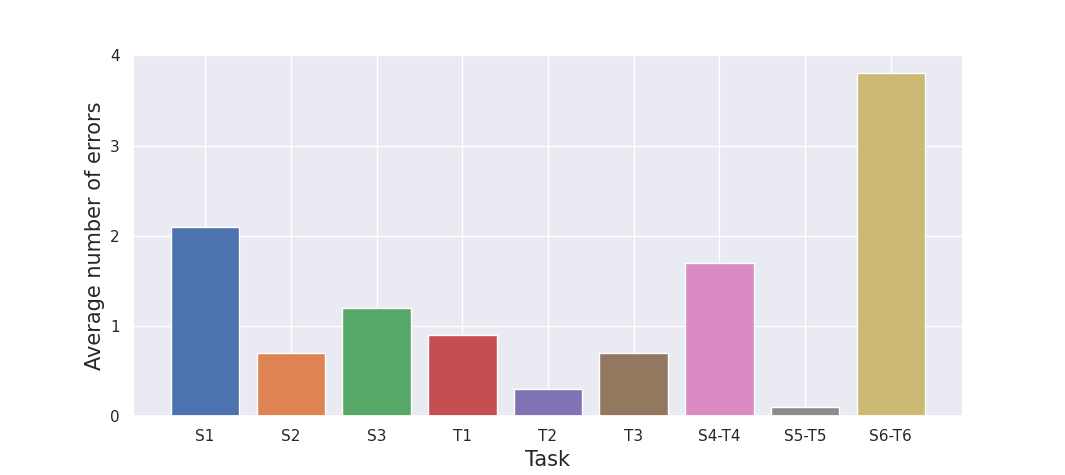
\includegraphics[width=1.2\textwidth]{images/BarsErrors.png}}%
            \captionsetup{justification=centering}
            \caption{Average of user errors for each task}
            \label{BarsErrors}
        \end{minipage}
    \end{figure}

\subsubsection{Task difficulty}
    % Task difficulty
    %   - Linee spezzate per ogni task, con una linea spessa per avg (tester, voto)


\subsection{Discussion of results}
    % Your observations on results
    % Summary of comments from user testing